\documentclass[tikz,border=12pt]{standalone}
\usepackage{tikz}
\usetikzlibrary{arrows.meta}
\begin{document}
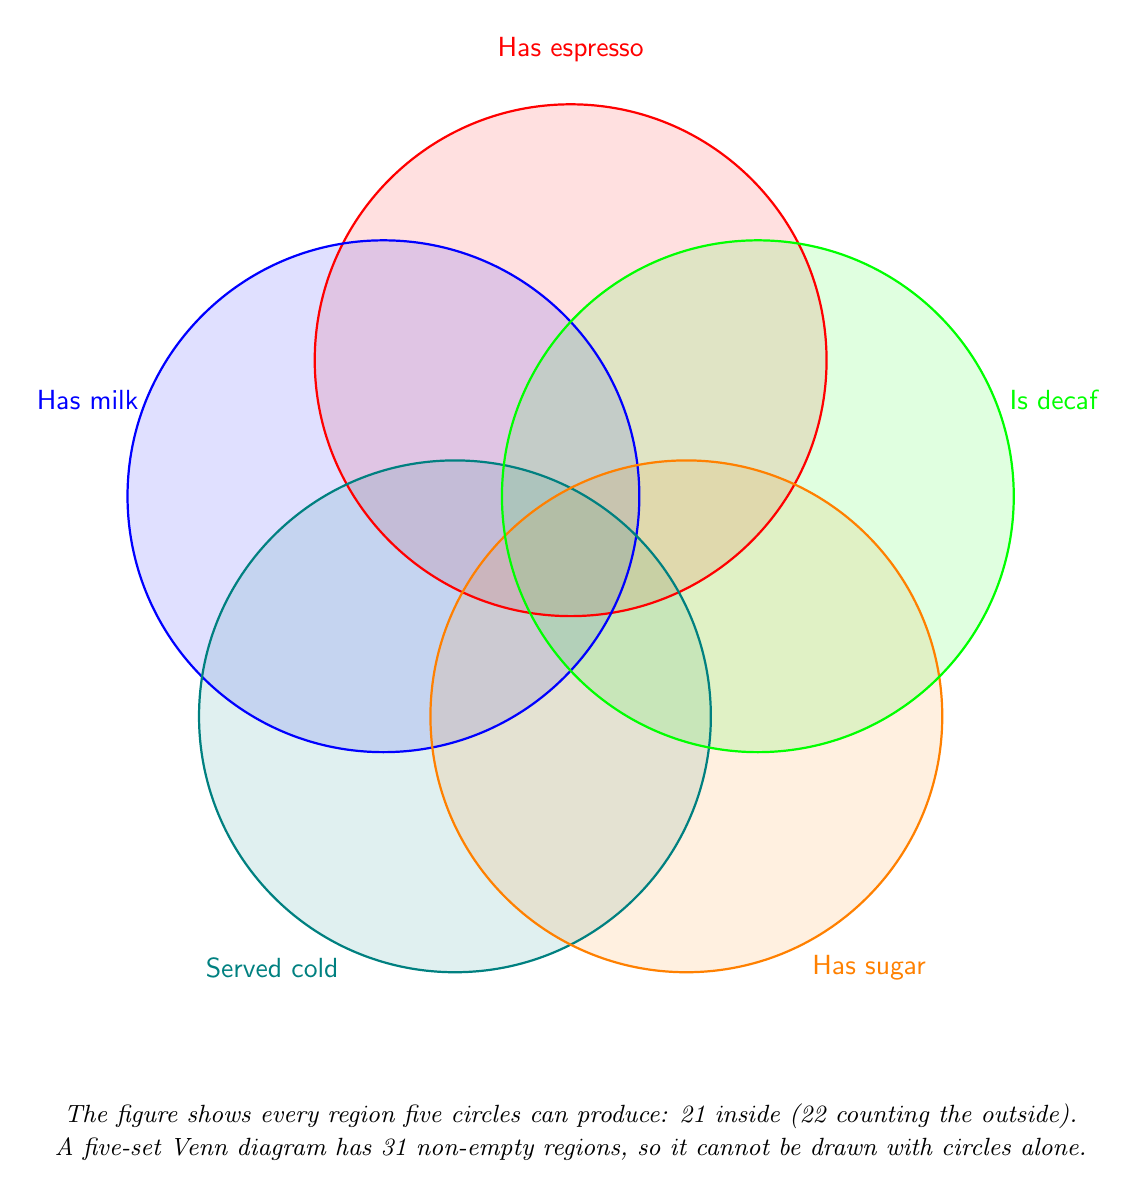
\begin{tikzpicture}[font=\sffamily]
  \def\Rc{2.5}
  \def\rad{3.25}

  % centres of the five circles, on a regular pentagon
  \coordinate (C1) at (90:\Rc);   % Has espresso
  \coordinate (C2) at (162:\Rc);  % Has milk
  \coordinate (C3) at (234:\Rc);  % Served cold
  \coordinate (C4) at (306:\Rc);  % Has sugar
  \coordinate (C5) at (18:\Rc);   % Is decaf

  \begin{scope}
    \fill[red,opacity=0.12]     (C1) circle (\rad);
    \fill[blue,opacity=0.12]    (C2) circle (\rad);
    \fill[teal,opacity=0.12]    (C3) circle (\rad);
    \fill[orange,opacity=0.12]  (C4) circle (\rad);
    \fill[green,opacity=0.12]   (C5) circle (\rad);
  \end{scope}

  \draw[red,thick]    (C1) circle (\rad);
  \draw[blue,thick]   (C2) circle (\rad);
  \draw[teal,thick]   (C3) circle (\rad);
  \draw[orange,thick] (C4) circle (\rad);
  \draw[green,thick]  (C5) circle (\rad);

  \node[red]    at (90:6.45)  {Has espresso};
  \node[blue]   at (162:6.45) {Has milk};
  \node[teal]   at (234:6.45) {Served cold};
  \node[orange] at (306:6.45) {Has sugar};
  \node[green]  at (18:6.45)  {Is decaf};

  \node[align=center,font=\small\itshape] at (0,-7.3)
    {The figure shows every region five circles can produce: 21 inside (22 counting the outside).\\[1pt]
     A five-set Venn diagram has 31 non-empty regions, so it cannot be drawn with circles alone.};
\end{tikzpicture}
\end{document}
